\documentclass{beamer}
\usepackage[utf8]{inputenc}
\usepackage{tikz}
\usepackage[export]{adjustbox}
\usepackage[americaninductors]{circuitikz}
%    \usepackage{biblatex}
 \usetikzlibrary{arrows}
\usepackage[T1]{fontenc}
\mode<presentation> {
\usetheme{Lisbon}
}

\usepackage{graphicx} % Allows including images
\usepackage{booktabs} % Allows the use of \toprule, \midrule and \bottomrule in tables

%----------------------------------------------------------------------------------------
%	TITLE PAGE
%----------------------------------------------------------------------------------------

\title[Adiabatic Switching and Reversible Logic in CMOS circuits]{Adiabatic Switching and Reversible Logic in CMOS circuits} 
\subtitle{Towards Low Energy Computing} 
\institute[IST] 
{
Physics of Classical and Quantum Information, 2017/18 \\
\medskip
Instituto Superior T\'{e}cnico, Universidade de Lisboa \\ 
\medskip
\textit{jose.leitao@tecnico.ulisboa.pt} 
}
\author{Jos\'{e} Leit\~{a}o }
\date{December 15, 2017} 

\begin{document}

%\logo{
\includegraphics[width=\dimexpr\textwidth-2\fboxrule-2\fboxsep,trim=150px 200px 150px 150px,clip]{logo_institute}}

\begin{frame}[plain]
\titlepage % Print the title page as the first slide
\end{frame}

\begin{frame}
\frametitle{Overview} % Table of contents slide, comment this block out to remove it
\tableofcontents 
\end{frame}

%----------------------------------------------------------------------------------------
%	PRESENTATION SLIDES
%----------------------------------------------------------------------------------------

\section{Introduction}
\begin{frame}
\frametitle{ Integrated Circuits}
\begin{minipage}{.75\textwidth}

\begin{itemize}
\item Based on the inverter (NOT gate),  many other logic gates may be directly derived by the association of additional NMOS and PMOS in series and/or in parallel. 

\item Modern processors are made of tens of millions of such digital gates integrated on a single microchip.

\item {\bf Energy efficiency }is a top concern for today's electronic systems, from both  the \underline{environmental} and  \underline{usability} point of views.  

\end{itemize}
\end{minipage}
\hfill
\begin{minipage}{.2\textwidth}
\begin{figure}
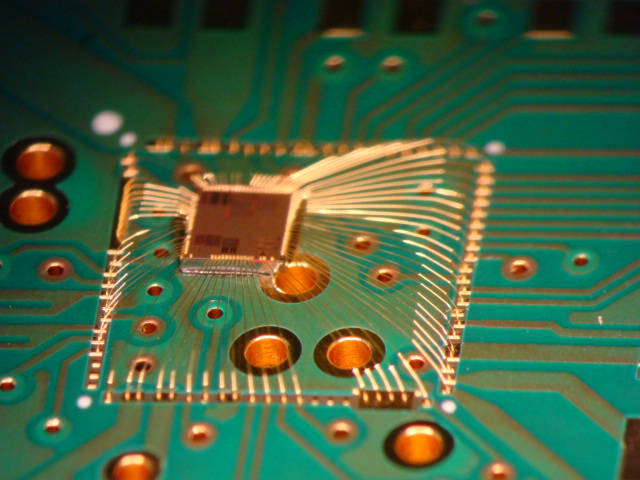
\includegraphics[width=1.3\linewidth]{img/ic3.jpg}
\\
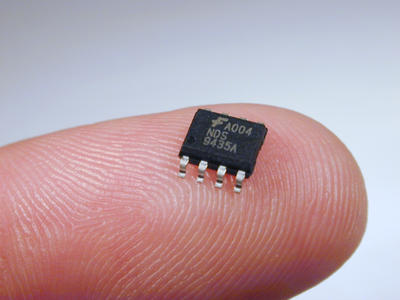
\includegraphics[width=1.3\linewidth]{img/ic2.jpg}

\end{figure}
\end{minipage}
\end{frame}

\section{Fundamental Theory }
\subsection{Adiabatic Logic}

\begin{frame}
\frametitle{Split-Charge Recovery Logic\footnote{\tiny S.Younis, \emph{Asymptotically zero energy computing using split-level charge recovery logic} , Ph.D. Dissertation, MIT, Cambridge,1994 }}

\begin{circuitikz}[scale=1,american voltages]
\draw[color=black,thick]
(2,0) node[nmos] (nmos1) {}
(2,2) node[pmos,emptycircle] (pmos1) {}
(nmos1.D) to [short,-*]++(0,0.25) node[right]{$\frac{V_{DD}}{2}$} to  (pmos1.D) 
(nmos1.S)  to [short,-o] ++(0,-0.5) node[below]{$V_{DD}/2$}
(pmos1.S)  to [short,-o] ++(0,0.5) node[above]{$V_{DD}/2$}
(nmos1.G) to [short] ++(0,1) to [short] ++(-0.5,0)  node[above,color=blue]{$A_1$}
(nmos1.G) to (pmos1.G)

(2.5,3) to (3.5,3) to (4,3.5) to (5,3.5) 
(2.5,-1) to (3.5,-1) to (4,-1.5) to (5,-1.5)  
 
(6,0) node[nmos] (nmos2) {}
(6,2) node[pmos,emptycircle] (pmos2) {}
(nmos2.D) to [short,-*]++(0,0.25) node[right,color=blue]{$\overline{A_1}$} to  (pmos2.D) 
(nmos2.S)  to [short,-o] ++(0,-0.5) node[below]{$V_{SS}$}
(pmos2.S)  to [short,-o] ++(0,0.5) node[above]{$V_{DD}$}
(nmos2.G) to [short] ++(0,1) to [short] ++(-0.5,0)  node[above]{$A_1$}
(nmos2.G) to (pmos2.G)

(6.5,3.5) to (7.5,3.5) to (8,3) to (9,3) 
(6.5,-1.5) to (7.5,-1.5) to (8,-1) to (9,-1)  
 
(10,0) node[nmos] (nmos2) {}
(10,2) node[pmos,emptycircle] (pmos2) {}
(nmos2.D) to [short,-*]++(0,0.25) node[right,color=blue]{} to  (pmos2.D) 
(nmos2.S)  to [short,-o] ++(0,-0.5) node[below]{$V_{DD}/2$}
(pmos2.S)  to [short,-o] ++(0,0.5) node[above]{$V_{DD}/2$}
(nmos2.G) to [short] ++(0,1) to [short] ++(-0.5,0)  node[above,color=orange]{$A_2$}
(nmos2.G) to (pmos2.G)

;
\end{circuitikz}

 \end{frame}


\subsection{Results}
\begin{frame}
\frametitle {Table }

Energy Consumption of 2400-stage inverter chain\footnote{\tiny J.Lim et a., \emph{nMOS Reversible Energy Recovery Logic for Ultra-low-energy Applications} , IEEE Journal of Solid-State Circuits, Vol.35, No. 6 ,2000 }:


\begin{table}
\begin{tabular}{l |cccl}
\toprule
 Implementation & 55 kHz & 250 kHz & 2 MHz \\
\midrule
Conventional CMOS & 27 pJ/cycle & 33.8 pJ/cycle & 40.2 pJ/cycle \\
Reversible CMOS  & 1.2 pJ/cycle & 4.3 pJ/cycle & 19.0 pJ/cycle  \\
\bottomrule
\end{tabular}
\end{table}
%\pause
\begin{itemize}
\item[\textcolor{green}{\checkmark}] Energy saving $\approx 2\times-22\times$
%\pause
\item[\textcolor{red}{$\times$}] Area overhead is significant (2$\times$)
%\pause

\item[\textcolor{orange}{\checkmark}] Might be suitable for energy-contrained applications (e.g: implants)

\end{itemize}
\end{frame}



\section{Conclusions}
\subsection{testt}
\begin{frame}
\frametitle{Conclusions}
\begin{itemize}
 \item Further research is required to clarify the practical application of this technology
 %\pause
\item (Classical) Reversible Computing is growing in interest from both the research and industrial communities
%\pause
\item Fundamental physical principles may provide game-changing hints to improve engineered systems, 
but 
  the physical reality often presents us with (hard-to-grasp) practical limitations in return
 \end{itemize}
  \end{frame}




\begin{frame}

{\Huge{\centerline{Thank you}}}
\vspace{2em}
{\small I would also like to acknowledge the support of everyone}

\end{frame}


\end{document} 
